\chapter{Enforcing stability of the model}
The topic of this chapter is how to enforce stability of the identified models.\\

Every time we perform an open-loop experiment, it is required that the system is BIBO stable. Otherwise, given a bounded input \( u(k) \), the output \( y(k) \) might diverge, and we would not be able to measure it. Physically, the system would be destroyed. 

The fact that a system is BIBO stable is a \textbf{strong indication} of the parameters! Therefore, adding this information to the problem allows for more \textbf{accurate} estimates, which means smaller PUIs in our SM identification context.\\

\section{Stability of a discrete-time LTI system}
The following statements are equivalent:
\begin{enumerate}
    \item \( G_p(z) = \frac{N(z, \theta)}{D(z, \theta)} \) is BIBO stable:
    
    \item \( D(z, \theta) \neq 0 \)   for all \( z \in \mathbb{C} \) such that \( |z| \geq 1 \).\\
    
    \textbf{Observation:} We note that stability depends only on the parameters appearing in the denominator, which in turn defines the poles of the system.
    \newpage
    \item \textbf{Jury's theorem}:\\
    Let's define the Jury array as follows: \\
    
    Given \( D(z,\theta) = 1 + a_1 z^{-1} + a_2
    z^{-2} + \cdots + a_n z^{-n} \), the Jury array is defined by:

\[
\begin{array}{*{7}{c}@{\hspace{10pt}}}
    a_n & a_{n-1} & a_{n-2} & \cdots & a_2 & a_1 & a_0 = 1 \\
    1 & a_1 & a_2 & \cdots & a_{n-2} & a_{n-1} & a_n \\
    c_{n-1} & c_{n-2} & c_{n-3} & \cdots & c_1 & c_0 &  \\
    c_0 & c_1 & c_2 & \cdots & c_{n-2} & c_{n-1} &  \\
    d_{n-2} & d_{n-3} & \cdots & d_1 & d_0 & & \\
    d_0 & d_1 & \cdots & d_{n-3} & d_{n-2} & & \\
    \vdots & \vdots & \vdots & \vdots &  &  &  \\
    q_2 & q_1 & q_0 & & & & 
\end{array}
\]


    where:
    \[
    c_{n-1} = \det\left( \begin{bmatrix}
        a_n & a_{n-1} \\
        1   & a_1
    \end{bmatrix} \right)
    \]
    \[
    c_{n-2} = \det\left( \begin{bmatrix}
        a_n & a_{n-2} \\
        1   & a_2
    \end{bmatrix} \right)
    \]
    and,
    \[
    d_{n-2} = \det\left( \begin{bmatrix}
        c_{n-1} & c_{n-2} \\
        c_0   & c_1
    \end{bmatrix} \right)
    \]
   \[
    d_{n-3} = \det\left( \begin{bmatrix}
        c_{n-1} & c_{n-3} \\
        c_0   & c_3
    \end{bmatrix} \right)
    \]

    in general,
           \[
    c_{n-j} = \det\left( \begin{bmatrix}
        a_n & a_{n-j} \\
        a_0 =1   & a_j
    \end{bmatrix} \right)
    \]
    and
         \[
    d_{n-j} = \det\left( \begin{bmatrix}
        c_{n-1} & c_{n-j} \\
        c_0   & c_{j-1}
    \end{bmatrix} \right)
    \]
    
    Visually, it can be seen in the following figure.
    \begin{figure}[H]
    \centering
    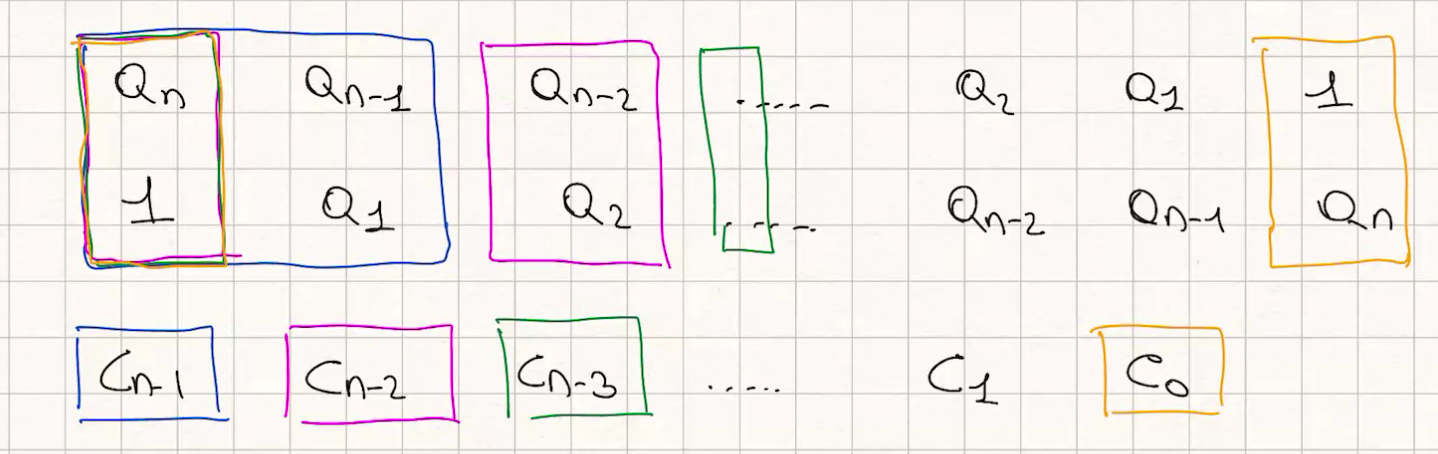
\includegraphics[width=0.75\textwidth]{jury-array.png}
    \caption{Shaping the third row of the Jury array of the aforementioned polynomial}
\end{figure}

    \textbf{Theorem (Jury)}:\\
    The roots of the polynomial $D(z,\theta)$ belongs to the open unit circle, which mathematically means \( D(z, \theta) \neq 0 \)   for all \( z \in \mathbb{C} \) such that \( |z| \geq 1 \), if and only if the following equations hold:
    \begin{itemize}
        \item\(
    D(z=1) = 1 + a_1 + a_2 + \cdots + a_n > 0
    \) 
        \item \((-1)^n D(z=-1) = (-1)^n (1 - a_1 + a_2 - a_3 + \cdots \pm a_n) >0\) 
        \item \(|a_n|<1 \)
        \item \(|c_{n-1}|< |c_0| \)
        \item \(|d_{n-2}| < |d_0|\)\\
        \vdots
        \item \(|q_2| < |q_0|\)
    \end{itemize}
    The first three inequalities are in $\theta$, while the others ones depending on the Jury array, can become non-linear, since we are dealing with the absolute values. In order to reformulate the problem in a form that can be handled in a linear fashion we adopt the following trick.
      \begin{itemize}
        \item \((c_{n-1})^2< (c_0)^2 \)
        \item \((d_{n-2})^2 < (d_0)^2\)\\
        \vdots
        \item \((q_2)^2 < (q_0)^2\)
    \end{itemize}
    These constraints now become \textbf{quadratic non-convex inequalities} in the elements of the Jury arrya. Moreover, the elements of the Jury array are \textbf{polynomial functions of $\theta$}, or at any rate we are dealing with determinent of two by two matricies, which leads to bilinear equations of the elements of the matrix.\\
    to conclude:
    \begin{itemize}
    \item We can enforce stability of the identified model by, \textbf{adding optimization variables representing the entried of the Jury array}, $c_{n-1},c_{n-2},\cdots,c_0,d_{n-2},\cdots,q2,q0 $, the definition of $q_1$ is not needed. Now we can modify the EFPS to include the:
     \item relations between $\theta$ and the entried of the Jury array \(a_1,\cdots,a_n \rightarrow c_{n-1},\cdots,c_0\)\\
     \item relations between different entried of the Jury array  \(c_{n-1},\cdots,c_0 \rightarrow d_{n-2},\cdots,d_0\) and so on up to $q_2$ and $q_0$\\
     \item Now, the equations from the Jury theorem.
    \end{itemize}
    \textbf{Remark:} even if we include these constraints, there is no guarantee that the final identified model will be stable, for the following reasons:
    \begin{itemize}
        \item we relax our POPs to convex SDP:
     \begin{figure}[H]
    \centering
    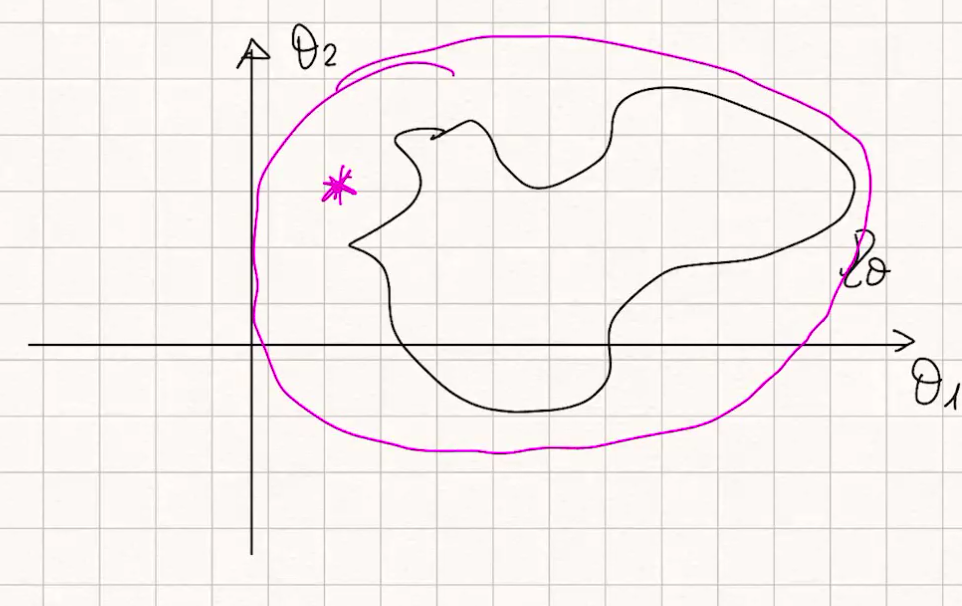
\includegraphics[width=0.75\textwidth]{SDP-convex-set.png}
    \caption{Since we relax our problem, the model obtained showed by * does not satisfies the stability property, since it does not satisfies all the constraints.}
\end{figure}
    \item Even if we could describe the exact FPS, then when taking the central estimate, we may \textbf{fall out of} the set, because our FPS is non-convex.
    \begin{figure}[H]
    \centering
    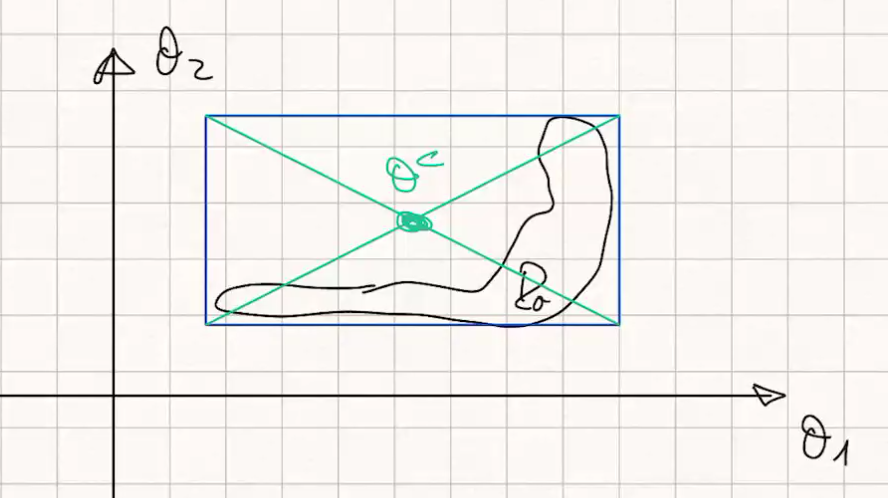
\includegraphics[width=0.5\textwidth]{centra-estimate.png}
    \caption{The central estimate that does not fall into the FPS.}
\end{figure}
    \end{itemize}
    So why enforcing stability constraints? since they shrink the FPS and ultimately improve the accuracy of the model because the obtained PUIs will be smaller.
\end{enumerate}

\begin{example}
\[
H(z) = \frac{\beta_1 z^{-1}}{1 + a_1 z^{-1} + a_2 z^{-2} + a_3 z^{-3}}
\]
we have the following Jury constraints
\[
D(z=1)> 0 \Rightarrow 1 + a_1 + a_2 + a_3 > 0
\]
\[
(-1)^nD(z=-1)> 0 \Rightarrow -1 + a_1 - a_2 + a_3 > 0
\]
\[
-1 <a3< 1
\]
Now, we need to shape Judy table, we need to go up to the third row, since the row with three element becomes the third row.
\[
\begin{array}{*{4}{c}@{\hspace{10pt}}}
    a_3 & a_2 & a_1 & 1 \\
    1 & a_1 & a_2 & a_3 \\
    c_2 & c_1 & c_0  
\end{array}
\]
where 
\[
c_2 = a_3 a_1 - a_2
\]
as it was mentioned $c_1$, here, is not needed.
\[
c_0 = a_3 a_3 - 1
\]
Now,
\[
|c_2|<|c_0| \Longleftrightarrow c_2^2 <c_0^2
\]

\end{example}

















